\documentclass[english]{retronlabo-manual}

\title{Retron 5: RetronLabo CFW Guide
\thanks{Thanks to ManCloud, Reminon and Stone}}
\author{\url{https://github.com/jayp76}}

\begin{document}

\maketitle

\begin{abstract}
This guide is about how to use the RetronLabo Custom Firmware for your Retron 5. It does not explain how to install or where to get it.
\todo{Add RetronLabo docs $\rightarrow$ ongoing}
\end{abstract}

\FrontMatter

\section{What's new and shiny in this firmware?}

This custom firmware brings a lot of features you'd find in a typical emulation box - except it's on your Retron 5! Meaning you also get all the cartridge and controller ports that has, making for a significantly better emulation box!

\subsection{Emulation Cores}

Old ones, new ones, alternative ones - this firmware supports emulation cores and loading newer, better, or just different ones for your favorite platforms. And that also means you can load some cores for platforms the Retron 5 was not made for, making it that much more versatile.

Different cores may work better with some games on platforms that are already supported, or they can support all new platforms, like \emph{PC-Engine} or \emph{Playstation}. The Sky's The Limit\footnote{You can actually prove that from a Computer Science standpoint - ignoring the practicalities of compiling compatible cores, which we're not getting into here, because... that's a longer document.}.

\subsection{Dump Your Own Cartridges}

Original carts are awesome, and they make for great collectors' items. But unfortunately, the systems natively supported by the Retron 5... aren't the youngest anymore. And even very simple circuit boards and ROM chips as used on those don't last forever. Just like the original hardware to run it on, those cartridges are getting older, and sooner or later they die. That's super frustrating when it's just the battery and you lose your precious Pokemon save file from when you were in high school - but it's also just plain sad when it happens to the ROM portion - cause it'll turn that OG copy of \emph{Shadowrun} into a weirdly shaped paperweight.

Fortunately, this firmware lets you remedy that: by allowing you to dump your cartridges and get a ROM file off it. (Saving the RAM was already a feature in the OG firmware, but yes, that too.)

Save your old cartridges - and hey, maybe you'll find you have a knack for ROM hacking. Now you can: with your own ROMs.

\subsection{Load Your Own ROMs}

Dumping carts would be a very moot feature without being able to load those ROMs again. So, yes: you can load your own ROMs.

Just be responsible. Don't get them from strange places - get from your own carts! You don't know where those other ones have been!

\todo{fit RetronLabo documentation onto SD Card and ship it with the firmware}

\section{Additional Files Used By Nonstandard Cores}

Remember when I said you might be able to run \emph{Playstation} games on your Retron? Well, there is one snag, which you might already be familiar with if you've dabbled with \emph{Playstation} emulation in the past: the BIOS.

See, the newer a console is, the more complex it is. And the more it's not just about having something that can emulate the hardware. The \emph{Playstation} is one of the first generation of consoles that didn't just stuff everything into magic hardware hooks. Instead, it has an honest to goodness, proper BIOS\footnote{Sorry, we're not counting \emph{ZX Spectrum}s, \emph{Amiga}s or \emph{Commodore 64}s and so on. They weren't consoles, they were home computers. Which also happened to be pretty ok at playing games. Yes those also have a ROM built into the device, much like a \emph{Playstation} BIOS, usually with a BASIC interpreter and somesuch - if you wanted to run those on your Retron 5, you would also need to get ahold of a copy of that ROM. Fair's fair.}. Incidentally, you may remember that from turning on your console and being greeted with a basic CD player and Memory Card editor.

So, ideally, you would hook a JTAG into your \emph{Playstation} and dump the BIOS yourself. Or hack PCSX-Reloaded enough to extract their open source BIOS? Or you happen to have a backup of that file, which is where the table \ref{tbl:bios-files} comes in.

\begin{figure}[h]
\caption{Screenshot of a folder view with BIOS files}
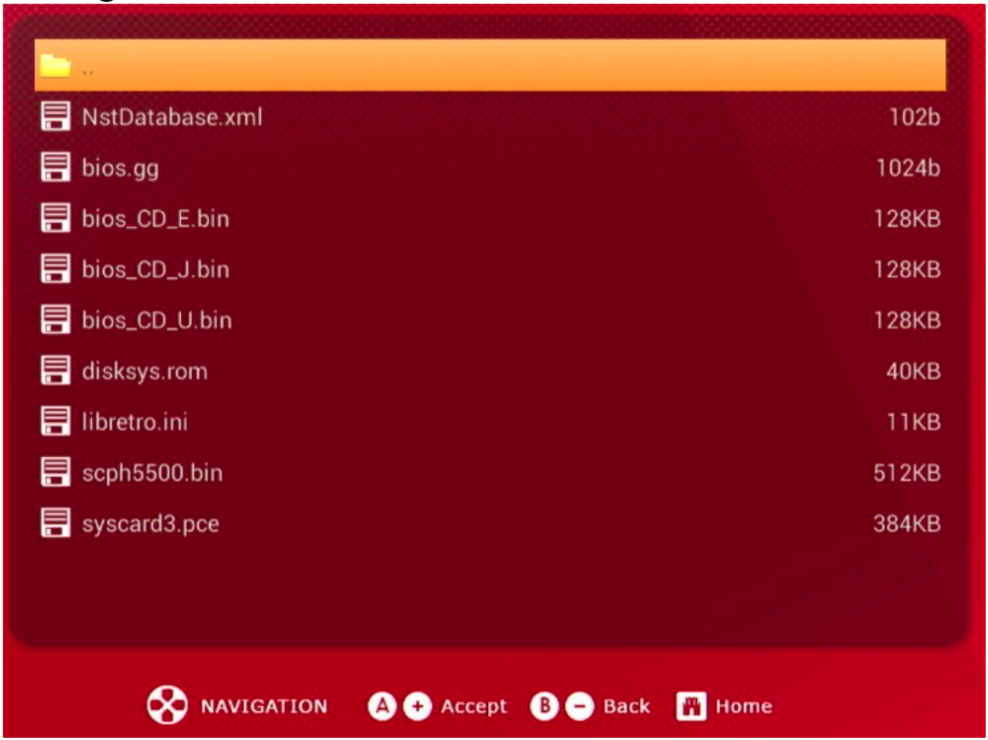
\includegraphics[width=\textwidth]{needed-files-for-alternate-cores}
\label{fig:needed-files-for-alternate-cores}
\floatfoot{The following files are listed: \texttt{NstDatabase.xml}, \texttt{bios.gg}, \texttt{bios\_CD\_E.bin}, \texttt{bios\_CD\_J.bin}, \texttt{bios\_CD\_U.bin}, \texttt{disksys.rom}, \texttt{libretro.ini}, \texttt{scph5500.bin}, \texttt{syscard3.pce.}}
\end{figure}

To retrofit your Retron with files like these - for any cores that may need them, whatever they are - you have to place them in the \texttt{\#Config} folder on your SD Card. You can then copy them through the Retron's menu to the \texttt{\#Internal Storage} of your device. You only need to do this once. The files will persist through reboots.

\clearpage

\subsection{\texttt{libretro.ini}: All Cores}

Guess what the firmware is using for those loadable cores? Yep: \emph{libretro}.

This file allows you to configure that library to some degree. Think controller input mapping and the like. And you must have some configuration to get started. Refer to the CFW thread if in doubt - which should also include a copy of that file tailored to the Retron 5.

\subsection{\texttt{bios.gg}: Game Gear}

The Game Gear needs its BIOS to be emulated properly. To make things more fun for everyone, that statement wasn't actually true for \emph{all} Game Gear releases: it's complicated. The BIOS you want to look for is commonly referred to as the \emph{Majesco} Game Gear BIOS - Majesco having re-issued Game Gears in the early 2000s, with Sega's blessing. While the BIOS was first noticed in these devices, it is actually also found on older Sega boards from as early as 1993. So: don't think about about the name too much.

It's a really fascinating story, and if you're curious about all the ins and outs check out the BIOS section on \emph{SMS Power}\footcite{ref:smsp-bios}. This should give you all the details you could ever want to know about Game Gear BIOSes.

\emph{RetronLabo}'s documentation does call out that it needs a BIOS file, so this is the one you want.

\subsection{\texttt{bios\_CD\_E.bin}, \texttt{bios\_CD\_J.bin}, \texttt{bios\_CD\_U.bin}: MegaDrive/MegaCD}

Each of the regions has its own BIOS, as you'd expect: PAL uses the \emph{E} version, Japan the \emph{J} and other NTSC regions the \emph{U}.

You may notice that in table \ref{tbl:bios-files} two of the files are stricken out. That's because, really, you only need one of them. They do not appear to be region locked, so you can just use whichever one of them you're most comfortable with and rename that to the others.

The US Mega CD BIOS may not load correctly, at least the one listed in the table did not. But since you can just use the Japanese one in its place, you'll probably be fine. If you do need to play musical chairs with the BIOS ROM image names, you may need to restart your \emph{Retron 5} and you may also need to delete your saved game snapshots for MegaCD games. BIOS ROM changes may affect some of the internal state of a console, thus by extension snapshots.

\subsection{\texttt{disksys.rom}: Famicom Disk System}

If you'd like to play FDS games, you'll need the bit of code that actually ran on the FDS. Because, unlike the Famicom itself, the Disk System actually had a bunch of stuff that was more complicated to handle. Thus this BIOS file.

It's basically the nice, cheerful \emph{Insert Disk} splash screen... and probably also the code that lets games write saves to the floppies. And of course the actual code to load stuff off of the floppies. If you've ever played an original FDS, you've probably come to appreciate its ability to load in extra stuff - although it does of course mean you'll have to occasionally flip the disk around. Well, it used to mean that. Now you have your Retron!

\subsection{\texttt{neogeo.zip}: NeoGeo through FBA (Counterexample)}

\emph{fbalpha} actually expects this nondescript ZIP file with related content in the same directory as the ROM you are trying to load. So, don't copy that into the internal storage on your Retron, leave it on the SD Card with your ROMs.

\subsection{\texttt{NstDatabase.xml}: Nintendo Entertainment System/Nestopia}

The \emph{Famicom Disk System} was quite a bit more sophisticated than the \emph{Famicom} that ran it - it turns out you do need some base programming to show a loading screen and access floppy drives.

If you'd like Nestopia to support FDS dumps, you will need a copy of this file. It doesn't actually provide anything like the aforementioned loader, because that would be pointless in context. Instead, it's a database file that lists ROM checksums and maps them to a bunch of metadata\footnote{Seriously, it's \texttt{CRC} and \texttt{SHA1} checksums mapped to region of the system and the correct mapper chip the ROM expects, along with chip size information. You'd expect that to be in the header - but I guess that might make those floppy images a bit awkward?} that is needed for full emulation of those ROMs - and is sadly not in any header information. Or at least not consistently.

This file is available from any \emph{Nestopia} source code archive, such as the \emph{libretro} one on GitHub\footcite{ref:libretro-nestopia}. The reason it's a separate file isn't for licensing so much as that it needs to be easy to update. More frequently than the emulation core itself.

\subsection{\texttt{scph5500.bin}: Playstation}

Funny how alphabetic sorting made the intro example one of the last subsections here.

The file name actually refers to the model number of the \emph{Playstation} the BIOS was loaded from: SCPH-5500 is the original Japanese \emph{Playstation 1}. Unlike the MegaCD, these are kind of region locked, however, meaning that - for better or worse - the file listed in table \ref{tbl:bios-files} is actually the US \texttt{scph5501.bin} but renamed to the Japanese model. That version of the BIOS will let you run games released outside of Japan.

\subsection{\texttt{syscard3.pce}: PC-Engine}

You only need this if you want to play CD games. And in fact, you could probably use many other versions, according to the documentation provided with the core, but \texttt{syscard3.pce} is the latest known (Japanese) 3.0 version of this BIOS. It should offer the most compatibility with CD based games.

Again, you do not need this for the floppy trading card looking games\footnote{They are apparently called \emph{HuCard}s. And seriously, they most definitely look like Pokemon trading cards.} - barring core bugs, of course.

\subsection{Reference BIOS File Checksums}

The files in table \ref{tbl:bios-files} are ones that have worked during testing and are thus known to be compatible. It's entirely possible that other BIOS versions for these systems will work just as well - but just in case they don't, try these files.

\begin{table}[hb]
\begin{tabular}[t]{|l|>{\ttfamily}l|>{\ttfamily}r|}
  \hline
  \multicolumn{1}{|l}{\bfseries System} & \multicolumn{1}{c}{\bfseries File} & \multicolumn{1}{c|}{\bfseries MD5} \\
  \hline
  Game Gear & bios.gg & 672E104C3BE3A238301ACEFFC3B23FD6 \\
  \multirow{3}{*}[1em]{MegaDrive/MegaCD} & \sout{bios\_CD\_E.bin} & \sout{7E146768A62DA68D771ED8B08079A5B5} \\
  & bios\_CD\_J.bin & 45DD7A6A87CA6AD4D0A54E8A2E3C097E \\
  & \sout{bios\_CD\_U.bin} & \sout{3B7D1CCA456F3CD7DFDF5C2711443D67} \\
  Nintendo Entertainment System & disksys.rom & C8B78295EB182F25C90DCD3DB9FA81EC \\
  Playstation & scph5500.bin & 924E392ED05558FFDB115408C263DCCF \\
  PC-Engine & syscard3.pce & C00A65C9CC8707F7202CD15A091C6A3F \\
  \hline
\end{tabular}
\captionof{table}{Known good BIOS files, with checksum}
\label{tbl:bios-files}
\end{table}

\section{Loading Cores}

All set up? Good! Here's what you do to load a shiny new core:

\say{Load Rom} $\rightarrow$ \say{\#Cores} $\rightarrow$ System e.g. FBA $\rightarrow$ libcore-xxx.so e.g. libcore-fba.so $\rightarrow$ \say{Copy}

\emph{Note}: the menu does not list any information about what cores are currently loaded. Neither here, nor anywhere else.

\todo{Maybe that needs fixing - the Retron 5 UI really could do with an overhaul.}

\subsection{Core Hygiene}

Cores are programs. Proper programs - they are the full emulators you're going to be using. Therefore, you should not run any random core you come across without at least some basic verification - they could be viruses, although they'd be rather limited on that console. Or they could be pranks written by jerks that just delete all your RAM backups. Don't run a core from a suspect source. \footnote{Yes, I see the irony given that this is a custom hacked firmware.}

\subsection{Persistence}

Loaded cores are not saved permanently. This means a simple reboot of your Retron 5 will unload all of them and return you to the default cores built into the system.

That's good and bad news: good news, because these cores - assuming they're genuine - won't brick your system. Because they don't stick around. The bad news is... you're going to have to load them every time you restart the console.

\subsection{Reboots}

You do not actually need to reboot to load a new core. Unless your console is kind of acting weirdly, in which case that reboot would unload anything that might be acting weird on your console.

Reboots are your magic reset button. All will be well.

\subsection{Cleaning Up After Cores}

If you happen to run into issues with loading a particular game with a particular core, try deleting the game from the internal storage and loading a different one.

The folder shown there can be found at \say{\texttt{\#Internal storage}/\texttt{CORE NAME}/\texttt{GAME NAME}} through the Menu. The screen should look like screenshot \ref{fig:unknown-game}.

\todo{Someone should port a database with game names for other consoles.}

You could also try deleting all save states. The Retron 5's original firmware has a tendency to create save states for just starting games - which gets awkward if you swap out the emulator underneath and it'll try to load a different emulator's save state. The Retron will do this even if you do not actually use save states, so it may be worth investigating.

\begin{figure}[ht]
\caption{Screenshot with Menu Options for a ROM.}
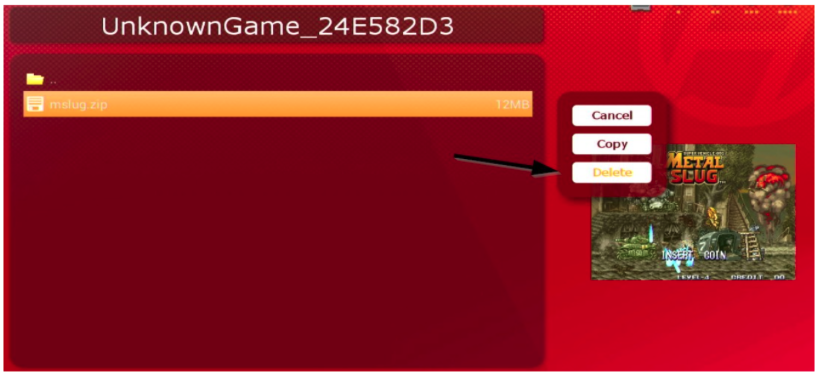
\includegraphics[width=\textwidth]{unknown-game}
\label{fig:unknown-game}
\floatfoot{Screenshot of a paused instance of Metal Slug. The System did not recognise the game file - this may mean you have a different version than the devs anticipated, or that the cartridge dump got corrupted. Note the arrow pointing to the \say{Delete} Menu Option, allowing you to recycle that space.}
\end{figure}

\section{Troubleshooting}

Back in the Good Old Days we used to blow the cartridge contacts if games acted up. This was a dumb idea: the moisture from the exhaled air causes corrosion of the game contacts. Don't do that. Despite this, that actually tended to work! What gives? Well, the mechanical act of reseating the game usually did the trick. Now you know how to fix that!

But how to deal with New Shiny Features acting up? Here's a few of the more likely scenarios and how to fix them.

\subsection{You've loaded a core, but loading games boots you back to the menu}

There's a good chance you either don't have the right BIOS available, or it got corrupted. Double check that you have actually installed all the necessart BIOS files for the core you're trying to use - see the section on additional files for cores above.

Don't forget to copy the BIOS files to the internal storage as described - it won't do you any good on your SD Card.

If it's not the BIOS files and you're certain the ROM is not corrupted, that core may just not work with that game very well.

\subsection{Game loads, but it's trippily glitchy}

As previously mentioned, the Retron 5 creates save states for just booting into any game. This may collide with alternative cores you may have loaded - for instance if you've previously played some NES game on your console with the standard emulation core that the Retron came with, and you now loaded the Nestopia core. The Nestopia core may get confused by this save state data and load into a weird state with it.

If you're not using save states\footnote{Save states as in the snapshot feature of the console. This is not the same as the battery-backed RAM of your games. The RAM image file format is typically the same across emulators for the same system, meaning your actual save games that you made with the game itself, like you would've on the original console, should be fine. If not: flash it to a cartridge with the original core and then load it again with the new one.}, the fastest solution here is to just reset the game. So that it will be booted up with the core you actually selected. And to not load save states across cores.

You should not need to reboot your Retron 5 for this.

\subsection{FBA game boots, has audio but screen is black}

Try the following setting:

\say{Settings} $\rightarrow$ \say{Video} $\rightarrow$ \say{Force Original Resolution} $\rightarrow$ \say{On}

Apparently this core does not like resizing.

\subsection{\emph{Playstation}: Audio starts cutting out during long play sessions}

This appears to be a problem with the \emph{Playstation} core. Try exiting and reloading the Save State, or manually creating one and loading that.

Barring that, if you've been saving to virtual memory cards, just restart the game entirely and load as normal.

\subsection{Game is running too fast}

The emulation cores are actually doing a pretty good job about their timing being very close to the original hardware - barring intentional overclock modes.

If you do notice a game running too fast, check the \say{Screen Refresh Rate} in the \say{Settings}. Sometimes the PAL/NTSC detection doesn't quite work, and many games actually work in both modes - except for timing differences.

\say{Screen Refresh Rate} defaults to \say{Match Game} which will try its best to detect what's appropriate for a game, but again, it's not perfect. Other options are \say{Force 60 Hz} for NTSC and \say{Force 60 Hz} for PAL.

An example of a game that is known to not work quite right with the default \say{Match Game} setting is the PAL release of \say{Ghost in the Shell} on \emph{Playstation}. It'll run too fast and may even crash the console. Since it's a PAL game, forcing 50 Hz fixes the speed issues and improves stability of the game.

\subsection{Game is not starting}

A bad automatic game start save state created by the Retron 5 can cause games to not load at all - or act weird, as mentioned above, if you switch cores.

The default save state should not be needed for anything, really, so you can just delete it which tends to fix most problems. These saves are stored on your SD card under \say{Retron/Saves/Snapshot/System}.

Similarly, manual saves are stored under \say{Retron/Saves/Snapshot/User} - although you could just not load them instead of deleting them. Then again, if you have manual saves and you get the game to boot by deleting the system snapshot, you could confirm if the save state was the real problem by trying to load some of your manual saves. For Science.

\glsaddallunused
\printglossary[title=File Formats, toctitle=Supported ROM File Formats, type=file-type, nonumberlist]

\section{Core-Specific Notes}

\subsection{MegaCD/SegaCD Core}

\subsubsection{CUE Files}

The \texttt{*.cue} file must have a full path to its accompanying \texttt{*.bin} file, which means you're going to have to adjust them manually with a text editor\footnote{\texttt{*.cue} files are plain text. You can edit them with \emph{Notepad} or any other editor.}.

Example CUE file:

\begin{lstlisting}[breaklines]
FILE "../../../../external_sd/Retron/Roms/Genesis/Batman Returns (Sega CD) (U).bin" BINARY
\end{lstlisting}

I suppose the bright side is, that you'll be able to split those two files up? If you wanted to?

Similarly if your image has separate files for the individual tracks on the CD, each track will need that path.

Example:

\begin{lstlisting}[breaklines=true]
FILE "../../../../external_sd/Retron/Roms/Genesis/Popful Mail/Popful Mail (USA) (Track 1).bin "BINARY TRACK 01 MODE1 / 2352
INDEX 01 00:00:00
FILE "../../../../external_sd/Retron/Roms/Genesis/Popful Mail/Popful Mail (USA) (Track 2).bin" BINARY TRACK 02 AUDIO
INDEX 00 00:00:00
INDEX 01 00:02:00
FILE "../../../../external_sd/Retron/Roms/Genesis/Popful Mail/Popful Mail (USA) (Track 3).bin" BINARY TRACK 03 AUDIO
INDEX 00 00:00:00
INDEX 01 00:02:00
FILE "../../../../external_sd/Retron/Roms/Genesis/Popful Mail/Popful Mail (USA) (Track 4).bin" BINARY TRACK 04 AUDIO
INDEX 00 00:00:00
INDEX 01 00:02:00
\end{lstlisting}

\subsubsection{SD Card Image Placement}

This core allows creating folders on your SD Card under \say{Retron5/Roms/Genesis} for additional structure and customisation as you see fit. Which is extra nice with those multi-file CUE/BIN sets mentioned earlier.

% \section{ROM Dumping}
\todo{Document how to actually dump your own carts to a ROM file.}

\BackMatter

\end{document}
